\documentclass{beamer}
\usepackage[utf8]{inputenc}
\usetheme{Copenhagen}
%\usepackage[spanish]{babel}
\usepackage{multirow}
%\usepackage{estilo-apuntes}
\usepackage{braids}
\usepackage[]{graphicx}
\usepackage{rotating}
\usepackage{pgf,tikz}
\usepackage{pgfplots}
\usepackage{tikz-cd}
\usepackage{mathtools}
%\usepackage{oplotsymbl} %filled pentagon go brrrr
%\usepackage{empheq}
%\usepackage[dvipsnames]{xcolor}
%\usepackage{xcolor}

\usetikzlibrary{arrows}
\usetikzlibrary{cd}
\usetikzlibrary{babel}
\pgfplotsset{compat=1.13}
\usetikzlibrary{decorations.shapes}
%\pgfkeyssetvalue{/tikz/braid height}{1cm} %no parece hacer nada
%\pgfkeyssetvalue{/tikz/braid width}{1cm}
%\pgfkeyssetvalue{/tikz/braid start}{(0,0)}
%\pgfkeyssetvalue{/tikz/braid colour}{black}

\theoremstyle{definition}

\newtheorem{theo}{Theorem}
\newtheorem{defi}{Definition}
\newtheorem{prop}[theo]{Proposition}
\newtheorem{lem}[theo]{Lemma}

\newcommand{\Z}{\mathbb{Z}}
\newcommand{\Q}{\mathbb{Q}}
\newcommand{\C}{\mathbb{C}}
\newcommand{\CC}{\mathcal{C}}
\newcommand{\OO}{\mathcal{O}}
\newcommand{\Tot}{\mathrm{Tot}}
\newcommand{\D}{\mathbb{D}}
\newcommand{\s}{\mathfrak{s}}
\providecommand{\gene}[1]{\langle{#1}\rangle}

\DeclareMathOperator{\im}{im}


\addtobeamertemplate{navigation symbols}{}{%
    \usebeamerfont{footline}%
    \usebeamercolor[fg]{footline}%
    \hspace{1em}%
    %\insertframenumber/\inserttotalframenumber
}
\setbeamercolor{footline}{fg=black}
\setbeamerfont{footline}{series=\bfseries}

\newcommand{\highlight}[1]{%
	\colorbox{red!50}{$\displaystyle#1$}}

\makeatletter
%\newcommand*{\encircled}[1]{\relax\ifmmode\mathpalette\@encircled@math{#1}\else\@encircled{#1}\fi}
%\newcommand*{\@encircled@math}[2]{\@encircled{$\m@th#1#2$}}
%\newcommand*{\@encircled}[1]{%
%	\tikz[baseline,anchor=base]{\node[draw,circle,outer sep=0pt,inner sep=.2ex] {#1};}}
%\makeatother


%-----------------------------------------------------------

\title{The derived Deligne conjecture}
\author{Javier Aguilar Mart\'in}
\institute{University of Kent}
\date{}
 
\begin{document}
\frame{\titlepage}

\begin{frame}
AVOID OPERADS

MOTIVATE AINFTY THROUGH TRANSFER (MAYBE) AND MINIMAL MODELS (MORE IMPORTANT)
REPRESENT THE RELATIONS WITH ASSOCIAHEDRA TO BE MORE VISUAL (AND TO PROVIDE AN EXAMPLE THROUGH CHAINS)
INFTY DELIGNE CONJECTURE (FIRST TIME COMPLETE LIST OF BRACE RELATIONS, PROBABLY KNOWN BUT DESCRIBED OTHER WAYS)
MOTIVATE DERIVED AINFTY ALGEBRAS (MENTION LACK OF GEOMETRICAL MODEL)
DERIVED DELIGNE CONJECTURE

\end{frame}
\begin{frame}
\tableofcontents
\end{frame}

\section{Algebraic Deligne Conjecture}
\begin{frame}
\begin{itemize}
\item<1-> Let $A$ be a graded $R$-module and consider the module $C^n(A)=\hom_R(A^{\otimes n},A)$.  %if you know about operads this is obvious, but I want to avoid them
\item<2-> For $f\in C^n(A)$ and $g_i\in C^{m_i}(A)$ define the \emph{brace} $b_j(f;g_1,\dots, g_j) \in C^{n+\sum m_i-j}(A)$ as
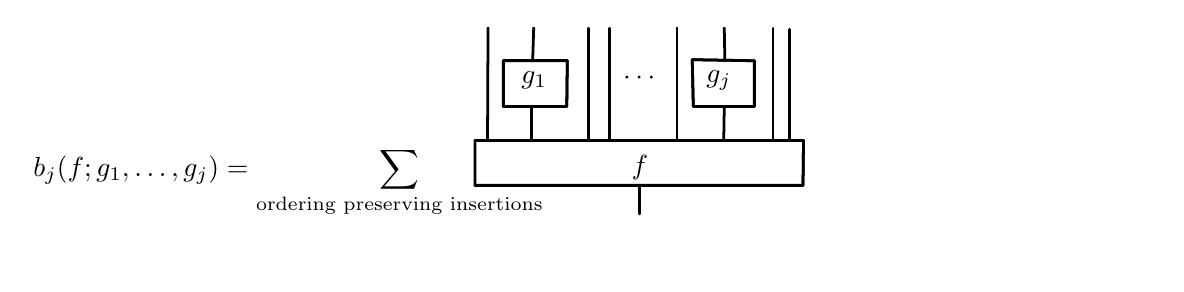
\begin{tikzpicture}[line cap=round,line join=round,>=triangle 45,x=1.0cm,y=1.0cm]
		\clip(-2.8466666666666676,-1) rectangle (11.486666666666668,2.);
		\draw[line width=1.pt] (2.833333333333334,0.) -- (2.833333333333334,0.5666666666666675) -- (7.006666666666668,0.5666666666666675) -- (7.,0.) -- cycle;
		\draw[line width=1.pt] (3.193333333333334,1.) -- (4.,1.) -- (4.006666666666668,1.58) -- (3.193333333333334,1.58) -- cycle;
		\draw[line width=1.pt] (6.,1.) -- (6.38,1.) -- (6.38,1.58) -- (5.593333333333335,1.5933333333333344) -- (5.606666666666667,1.) -- cycle;
		\draw (-2.9,0.6) node[anchor=north west] {$b_j(f;g_1,\dots, g_j)=\displaystyle{\sum_{\text{ordering preserving insertions}}}$};
		\draw [line width=1.pt] (2.833333333333334,0.)-- (2.833333333333334,0.5666666666666675);
		\draw [line width=1.pt] (2.833333333333334,0.5666666666666675)-- (7.006666666666668,0.5666666666666675);
		\draw [line width=1.pt] (7.006666666666668,0.5666666666666675)-- (7.,0.);
		\draw [line width=1.pt] (7.,0.)-- (2.833333333333334,0.);
		\draw [line width=1.pt] (4.92,0.)-- (4.92,-0.36666666666666614);
		\draw [line width=1.pt] (2.993333333333334,0.5666666666666675)-- (3.,2.);
		\draw [line width=1.pt] (3.553333333333334,0.5666666666666675)-- (3.553333333333334,1.);
		\draw [line width=1.pt] (4.273333333333334,0.5666666666666675)-- (4.273333333333334,1.9933333333333345);
		\draw [line width=1.pt] (4.54,0.5666666666666675)-- (4.54,1.9933333333333345);
		\draw [line width=1.pt] (5.993333333333334,0.5666666666666675)-- (6.,1.);
		\draw [line width=1.pt] (6.62,0.5666666666666675)-- (6.62,1.9933333333333345);
		\draw [line width=1.pt] (6.833333333333335,0.5666666666666675)-- (6.833333333333335,1.98);
		\draw [line width=1.pt] (3.193333333333334,1.)-- (4.,1.);
		\draw [line width=1.pt] (4.,1.)-- (4.006666666666668,1.58);
		\draw [line width=1.pt] (4.006666666666668,1.58)-- (3.193333333333334,1.58);
		\draw [line width=1.pt] (3.193333333333334,1.58)-- (3.193333333333334,1.);
		\draw [line width=1.pt] (6.,1.)-- (6.38,1.);
		\draw [line width=1.pt] (6.38,1.)-- (6.38,1.58);
		\draw [line width=1.pt] (6.38,1.58)-- (5.593333333333335,1.5933333333333344);
		\draw [line width=1.pt] (5.593333333333335,1.5933333333333344)-- (5.606666666666667,1.);
		\draw [line width=1.pt] (5.606666666666667,1.)-- (6.,1.);
		\draw [line width=1.pt] (3.5666666666666673,1.58)-- (3.58,2.);
		\draw [line width=1.pt] (6.007451656136321,1.586314378709553)-- (6.,2.);
		\draw [line width=1.pt] (5.4,0.5666666666666675)-- (5.4,2.);
		\draw (3.3,1.5666666666666678) node[anchor=north west] {$g_1$};
		\draw (5.65,1.58) node[anchor=north west] {$g_j$};
		\draw (4.7,0.5) node[anchor=north west] {$f$};
		\draw (4.59,1.5533333333333343) node[anchor=north west] {$\cdots$};
		\end{tikzpicture}
\item<3-> Notation: $b_1(f;g)=f\circ g = \sum_i f\circ_i g$.
\end{itemize}
\end{frame}

\subsection{Hochschild complex}
\begin{frame}
\frametitle{Hochschild complex of an associative algebra}
For $f\in C^n(A)$ let $|f|=\deg(f)+n-1$.\pause
\begin{lem}
The operation $[f,g]=f\circ g-(-1)^{|f|}g\circ f$ defines a Lie bracket on $C^*(A)$. 
\end{lem}\pause

\begin{defi}
Let $A$ be a dg algebra. Its \emph{Hochschild complex} $C^*(A)$ is given by $C^n(A)=\hom_R(A^{\otimes n},A)$ with the differential %I like C^0 as R -> A
\[
D(f) = [d+m,f] = d\circ f - (-1)^{|f|}f\circ d + m\circ f - (-1)^{|f|}f\circ m %the jacobi identity guarantees that this is a differential
\]
where $d$ and $m$ are the differential and multiplication on $A$.
\end{defi}

\end{frame}

\begin{frame}
\begin{itemize}
\item $C^*(A)$ is also a dga with multiplication %so we can consider its Hochschild complex and it has brace structure etc
\[
M(f_1,f_2) = (-1)^{|f|}b_2(m;f_1,f_2).
\]
\end{itemize}\pause
\begin{prop}[Gerstenhaber-Voronov]
The map $C^*(A)\to C^*(C^*(A))$ given by 
\[
x\mapsto \sum_{j\geq 0} b_j(x;-)
\]
is a map of dgas.
\end{prop}
\end{frame}


\subsection{Deligne conjecture}
\begin{frame}
\frametitle{Algebraic Deligne conjecture}
%When you unravel what the above means
\begin{theo}[Gerstenhaber-Voronov]
 The Hochschild complex $C^*(A)$ has the structure of a \emph{homotopy $G$-algebra}:\pause
 \begin{align*}
 b_j(m(f_1,&f_2);g_1,\dots,g_j) = \\
 &\sum_{k=0}^j (-1)^\varepsilon m(b_k(f_1;g_1,\dots, g_k),b_{j-k}(f_2;g_{k+1},\dots, g_j))
 \end{align*}
 %varepsilon is the koszul sign
 and
\end{theo}
\end{frame}
\begin{frame}
\begin{block}{}
 \begin{align*}
&b_j(D(f);g_1,\dots, g_j)-D(b_j(f;g_1,\dots,g_j))\\
-&(-1)^{|f|+1}\sum_{p=1}^j(-1)^{\sum_{i=1}^p|g_i|}b_j(f;g_1,\dots,D(g_p),\dots, g_j)\\
=&-(-1)^{(|f|+1)|g_1|}M(g_1,b_{j-1}(f;g_2,\dots, g_j))\\
 &+(-1)^{|f|+1}\sum_{p=1}^{j-1}(-1)^{j-1+\underset{i=1}{\overset{p}{\sum}}|g_i|}b_{j-1}(f;g_1,\dots,M(g_p,g_{p+1}),\dots g_j)\\
 &-(-1)^{|f|+\sum_{i=1}^{j-1}|g_i|}M(b_{j-1}(f;g_1,\dots, g_{j-1}),g_j)
\end{align*}
\end{block}
\end{frame}


\begin{frame}
MAYBE ALSO STRUCTURE ON COHOMOLOGY
\end{frame}

\section{$A_\infty$-algebras}


\begin{frame}
\frametitle{$A_\infty$-algebras}
\begin{defi}
An $A_\infty$-\emph{algebra} $A$ is an $R$-module equipped with a family of ``multiplications'' $m_n:A^{\otimes n}\to A$ of degree $2-n$ satisfying the relation %MAYBE CHANGE CHAINS TO COCHAINS TO KEEP THE DEGREE 2-N, I WILL HAVE TO USE OPERADIC DESUSPENSION IN THIS CASE

\[\sum_{r+s+t\geq 1}(-1)^{rs+t}m_{r+1+t}(1^{\otimes r}\otimes m_s\otimes 1^{\otimes s})=0\] %we are composing every map with itself
\end{defi}
\end{frame}


\begin{frame}
\frametitle{Some particular cases}
\begin{itemize}
\item<1-> We always have $m_1m_1=0$, so in particular $A$ is a cochain complex.%CAN BE DEFINED ON THE CATEGORY OF CHAIN COMPLEX
\item<2-> If $m_i=0$ for $i\neq 2$, the relation becomes $m_2(1\otimes m_2)=m_2(m_2\otimes 1)$, so $A$ is an associative algebra.
\item<3->  We also have the relation \[m_1m_2=m_2(m_1\otimes 1)+m_2(1\otimes m_1)\]%DG %MONOID IN CHAIN COMPLEX ANALOGUE TO MONOID IN K-VECT
\item[]<4-> This is the Leibniz rule, and $A$ is a dga.
\end{itemize}
\end{frame}


\begin{frame}
\frametitle{$A_\infty$-algebras are homotopy associative algebras.}
%how do they generalize associative algebras
\begin{itemize}
\item<1-> For $r+s+t=3$ we have the relation
\begin{align*}
&m_2(m_2\otimes 1)-m_2(1\otimes m_2)=\\ %the failure of m_2 to be associative
&m_1m_3+m_3(m_1\otimes 1\otimes 1)+m_3(1\otimes m_1\otimes 1)+m_3(1\otimes 1\otimes m_1)
\end{align*}
\item[]<2-> $m_2$ is homotopy associative with homotopy given by $m_3$. %recall that m1 is a differential so on homology this vanishes
\item<3-> The higher relations are a homotopy coherent extension of this fact. %m3 satisfies some relation up to homotopy given by m4 and so on
\end{itemize}
\end{frame}

\begin{frame}
MAYBE GEOMETRIC INTERPRETATION
\end{frame}


\begin{frame}
\frametitle{Morphisms of $A_\infty$-algebras}
\begin{defi}
An \emph{$\infty$-morphism} of $A_\infty$-algebras $A\to B$ is a family of maps \[f_n:A^{\otimes n}\to B\] of degree $n-1$ satisfying for all $n\geq 1$ the equation
\begin{align*}
\sum_{r+s+t=n} (-1)^{rs+t}f_{r+1+t}(1^{\otimes r} \otimes m^A_s\otimes 1^{\otimes t})=\\
\sum_{i_1+\cdots+i_k=n} (-1)^s m^B_k(f_{i_1}\otimes\cdots\otimes f_{i_k}),
\end{align*}
where
$s=\sum_{\alpha<\beta}i_\alpha(1-i_\beta)$.%The composition of $\infty$-morphisms $f:A\to B$ and  $g:B\to C$ is given by 
%
%\[(gf)_n=\sum_r\sum_{i_1+\cdots+i_r=n}(-1)^s g_r(f_{i_1}\otimes\cdots
%\otimes f_{i_r}).\]
\end{defi}

\end{frame}
\begin{frame}
\begin{itemize}
\item<1-> We have $f_1m_1 = m_1f_1$, i.e. $f_1$ is a morphism of complexes.
\item<2-> We have
\[
f_1m_2 = m_2 (f_1\otimes f_1) + m_1f_2 + f_2 (m_1\otimes 1 + 1\otimes m_1),\]
which means that $f_1$ commutes with the multiplication $m_2$ up to a homotopy
given by $f_2$.
\end{itemize}
\end{frame}

\subsection{Minimal models}
\begin{frame}
\frametitle{Minimal models}
\begin{itemize}
\item An $A_\infty$-algebra is \emph{minimal} if $m_1 = 0$. 
\end{itemize}\pause
\begin{theorem}[Kadeishvili]
\begin{itemize}
\item If $A$ is a dga over a field, its cohomology $H^*(A)$ is a minimal $A_\infty$-algebra with multiplication $m_2$ induced by the multiplication on $A$.
\item There is an $\infty$-morphism of $A_\infty$-algebras $f:H^*(A)\to A$ such that $f_1$ is a quasi-isomorphism.
\item Under certain homological conditions, any other dga $A'$ with $H^*(A')\cong H^*(A)$ is quasi-isomorphic to $A$. 
\end{itemize}
\end{theorem}\pause
The $A_\infty$-algebra $H^*(A)$ is called the \emph{minimal model} of $A$. %This will be relevant later
%nice enough = HH(A,A) vanishes on degree 2-n %Replaced  means equivalent  %essentially = up to quasi-iso
%We would like to extend this result to a ground ring that is not necessarily a field.
\end{frame}

\subsection{Hochschild complex}
\begin{frame}
\frametitle{Structure on the Hochschild complex}
Let $C^*(A)$ be the Hochschild module of $A$. %it can be turned into a complex with m1 but I'm not doing that because there's a better one
\begin{itemize}
\item<1-> Define a new circle operation for $f\in C^n(A)$ and $g\in C^m(A)$ %it has a reason but i'm not talking about operads
\[f\tilde{\circ}_ig=(-1)^{(n-1)\deg(g)+(n-i)(m-1)}f\circ_i g.\]
\item<2-> Applied to  $A_\infty$-maps 
\[m_{r+1+t}\tilde{\circ}_{r+1}m_s=(-1)^{rs+t}m_{r+1+t}\circ_{r+1}m_s\]
\item[]<3-> The sign of the $A_\infty$-equation!
\end{itemize}
\end{frame}



\begin{frame}
\begin{itemize}
\item<1-> This simplifies the equation to
\[\sum_{r+s+t=n}m_{r+1+t}\tilde{\circ}_{r+1}m_s=0\] %but we can simplify it even more
\item<2-> Let $a\tilde{\circ}b=\sum_{i}a\tilde{\circ}_ib$ and let $m=m_1+m_2+\cdots$. The equation becomes just
\item[]<3-> \[m\tilde{\circ}m=0.\]
\end{itemize}
\end{frame}

\begin{frame}
\begin{itemize}
\item<1-> Since $m\tilde{\circ}m=0$, the Jacobi identity implies that $[m,[m,]]=0$ for the bracket induced by $\tilde{\circ}$.
\item<2-> Since $|m|=1$ map $[m,]:C^*(A)\to C^*(A)$ turns $C^*(A)$ into a cochain complex.
\item<3-> Indeed, it is possible to define an $A_\infty$-algebra structure on $C^*(A)$. %i don't have time for details
\end{itemize}
\end{frame}
\begin{frame}
\frametitle{$A_\infty$-multiplications}
\begin{prop}[Getzler]
Up to shifts, the following maps define an $A_\infty$-algebra structure on $C^*(A)$
\begin{align*}
&M_1(f)=[m,f]\\
&M_j(f_1,\dots, f_j)=\tilde{b}_j(m;f_1,\dots, f_j) %the brace induced by the new circle
\end{align*}
%generalices the associative result
\end{prop}\pause

\begin{prop}[Hinted at by Gerstenhaber-Voronov]
The map $\Phi:C^*(A)\to C^*(C^*(A))$ given by $Phi(x)= \sum_{j\geq 0} b_j(x;-)$ satisfies for all $j$
\[\Phi(M_j) = M_j(\Phi^{\otimes j})\]
%generalices the associative result
\end{prop}
\end{frame}


\subsection{Deligne conjecture}
\begin{frame}
\frametitle{$A_\infty$-Deligne conjecture}
\begin{theorem} %some structure was already known, but no complete set of brace relations 
The Hochschild complex $C^*(A)$ has the structure of a $J$-algebra:
\begin{align*}
\tilde{b}_n&(M_j(f_1,\dots, f_j);g_1,\dots, g_n)=\\
&\sum_{\mathclap{l,i_1,k_1,\dots, i_j,k_j}}(-1)^{\varepsilon}M_l(g_1,\dots, \tilde{b}_{k_1}(f_1;g_{i_1},\dots),\dots, \tilde{b}_{k_j}(f_j;g_{i_j},\dots),\dots, g_n).\\ 
\\
&\tilde{b}_j(M_1(f);g_1,\dots, g_j)=\\
&\sum_{l,k,i_1}(-1)^{\varepsilon}M_l(g_1,\dots, \tilde{b}_{k}(f;g_{i_1},\dots),\dots, g_j)\\
&-(-1)^{|f|}\sum_{l,k,i_1} (-1)^{\eta} \tilde{b}_k(f;g_1,\dots, M_l(g_{i_1},\dots,), \dots, g_j)
\end{align*}
\end{theorem}
\end{frame}



\section{Homotopy associativity}



\begin{frame}
The product $m$ is homotopy associative if $m(m\times 1)\simeq m(1\times m)$\pause 


\[\Downarrow\] 

\begin{center}
There is a map $M_3:[0,1]\times X^3\to  X$ such that 
\end{center}

\[M_3(0,x,y,z)=(xy)z \text{ and }M_3(1,x,y,z)=x(yz)\]
\end{frame}

\begin{frame}[fragile]
\frametitle{Homotopy coherence}
Product of 4 elements
\[
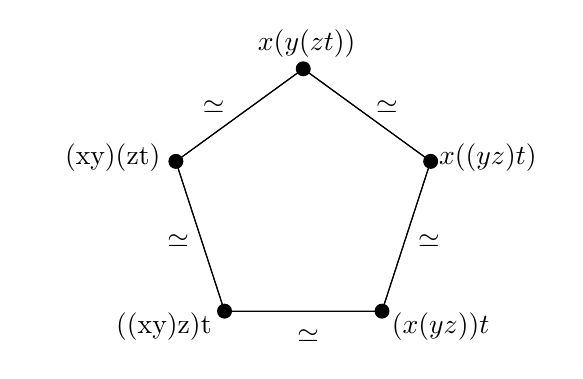
\begin{tikzpicture}[line cap=round,line join=round,>=triangle 45,x=1.0cm,y=1.0cm]
\clip(-1.5,0.5) rectangle (5.2,4.6);
\draw(1.,1.) -- (3.,1.) -- (3.618033988749895,2.9021130325903064) -- (2.,4.077683537175253) -- (0.3819660112501053,2.9021130325903073) -- cycle;
\draw (1.,1.)-- (3.,1.);
\draw (3.,1.)-- (3.618033988749895,2.9021130325903064);
\draw (3.618033988749895,2.9021130325903064)-- (2.,4.077683537175253);
\draw (2.,4.077683537175253)-- (0.3819660112501053,2.9021130325903073);
\draw (0.3819660112501053,2.9021130325903073)-- (1.,1.);
\draw (1.3,4.7) node[anchor=north west] {$x(y(zt))$};
\draw (3.6,3.25) node[anchor=north west] {$x((yz)t)$};
\draw (3,1.1) node[anchor=north west] {$(x(yz))t$};
\draw (-0.5,1.1) node[anchor=north west] {((xy)z)t};
\draw (-1.15,3.25) node[anchor=north west] {(xy)(zt)};
\draw (2.8,3.8) node[anchor=north west] {$\simeq$};
\draw (3.3333333333336,2.1) node[anchor=north west] {$\simeq$};
\draw (1.8,0.8933333333333304) node[anchor=north west] {$\simeq$};
\draw (0.15,2.1) node[anchor=north west] {$\simeq$};
\draw (0.6,3.8) node[anchor=north west] {$\simeq$};
\begin{scriptsize}
\draw [fill=black] (1.,1.) circle (2.5pt);
\draw [fill=black] (3.,1.) circle (2.5pt);
\draw [fill=black] (3.618033988749895,2.9021130325903064) circle (2.5pt);
\draw [fill=black] (2.,4.077683537175253) circle (2.5pt);
\draw [fill=black] (0.3819660112501053,2.9021130325903073) circle (2.5pt);
\end{scriptsize}
\end{tikzpicture}
\]

%If we can fill the pengaton with a homotopy $M_4=\pentagofill\times X^4\to X$ we say that the product is homotopy coherent. %there is a concatenation of homotopies and it makes sense to talk about homotopies between them, joining the points with paths
\end{frame}
\subsection{Stasheff Associahedra}

\begin{frame}
\frametitle{Associahedra}
Multiplying 5 elements
\[
\begin{tikzpicture}[line cap=round,line join=round,>=triangle 45,x=1.0cm,y=1.0cm]
\clip(-3.63,-1.8) rectangle (4.,3);
\draw(-0.5,0.) -- (0.,0.5) -- (-0.5,1.) -- (-1.,0.5) -- cycle;
\draw (-0.5,0.)-- (0.,0.5);
\draw (0.,0.5)-- (-0.5,1.);
\draw (-0.5,1.)-- (-1.,0.5);
\draw (-1.,0.5)-- (-0.5,0.);
\draw (-0.5,1.)-- (-0.76,2.87);
\draw (-0.76,2.87)-- (-2.13,1.59);
\draw (-2.13,1.59)-- (-1.98,0.82);
\draw (-2.13,1.59)-- (-2.5,1.);
\draw (-2.5,1.)-- (-2.31,0.29);
\draw (-2.31,0.29)-- (-1.98,0.82);
\draw (-1.98,0.82)-- (-1.,0.5);
\draw (0.,0.5)-- (0.93,0.89);
\draw (0.93,0.89)-- (0.98,1.68);
\draw (1.37,1.06)-- (0.98,1.68);
\draw (-0.76,2.87)-- (0.98,1.68);
\draw (-2.31,0.29)-- (-0.62,-1.3);
\draw (-0.5,0.)-- (-0.62,-1.3);
\draw (-0.62,-1.3)-- (1.22,0.35);
\draw (0.93,0.89)-- (1.22,0.35);
\draw (1.22,0.35)-- (1.37,1.06);
\draw [dash pattern=on 2pt off 2pt] (-2.5,1.)-- (1.37,1.06);
\end{tikzpicture}
\]

\end{frame}
\subsection{$A_\infty$-spaces}
\begin{frame}
\begin{itemize}
\item<1-> %We get spaces $K_2=*$, $K_3=[0,1]$, $K_4=\pentagofill$, $K_5, \dots$ %a point cause there is only one way to multiply two elements, [0,1] parametrizes the homotopy, k5 is the previous slide
\item<2-> And maps $M_n:K_n\times X^n\to X$ satisfying certain relations. %homotopy relation similar to what we explain with the polygons
\item<3-> For instance, $M_3:[0,1]\times X^3\to X$ defines a homotopy between $M_2(M_2\times 1)$ and $M_2(1\times M_2)$. 
\item<4-> $M_4:K_4\times X^4\to X$ allows us to fill the pentagon, on the boundary it is equal to $M_3$. %and so on
\end{itemize}
\end{frame}




\begin{frame}
\frametitle{Operad of $A_\infty$-algebras}
%FORMULATE THIS DIFFERENTLY SINCE I HAVE ALREADY OBTAINED THE OPERAD OF AINFTY ALGEBRAS THIS SHOULD BE JUST WRITING IT DOWN EXPLICITLY AND THEN ENCODE IT WITH OPERADIC SUSPENSION (PROBABLY JUST TELL THE RESULT OF INSERTIONS AND DEGREE BECAUSE THERE IS NO TIME TO EXPLAIN IT ALL)
\begin{itemize}
\item<1-> The operad $C^*(K)$ is generated by $m_n$ with $m_n\in C^*(K_n)$ for $n\geq 2$ and $m_1=\partial$ such that 
\[\sum_{r+s+t\geq 1}(-1)^{rs+t}m_{r+1+t}\circ_{r+1}m_s=0\]

\item<2-> We would like to obtain the signs directly from operadic composition.
\end{itemize}
\end{frame}
\subsection{Operadic suspension}
\begin{frame}
\frametitle{Operadic suspension}
\begin{itemize}
\item<1-> For a graded vector space $V=\bigoplus_{n\in\Z} V_i$ there is a \emph{suspension} operation $\Sigma V$ such that $(\Sigma V)_i=V_{i+1}$. \item<2-> $\Sigma V=V\otimes \mathbb{F}[-1]$.
\item<3-> We define an analogue of suspension for operads.
\end{itemize}
\end{frame}

\begin{frame}
\frametitle{Operadic suspension}
\begin{itemize}
\item<1-> Define $\Lambda(n)$ to be a 1-dimensional graded vector space concentrated in degree $n-1$.
\item<2-> The \emph{operadic suspension} $\mathfrak{s}\mathcal{O}$ of an operad $\mathcal{O}$ is given by $\mathfrak{s}\mathcal{O}(n)=\mathcal{O}(n)\otimes \Lambda(n)$ and composition maps determined by the following fact
\item[]<3->
\begin{theorem}[Markl]
There is an isomorphism of operads
\[ \mathfrak{s}End_{\Sigma V}\cong End_V\]
\end{theorem}
%\item<1-> Let $\Lambda(n)$ be a graded vector space concentrated in degree $1-n$ and generated by $e^n=e_1\land\cdots\land e_n$.
%\item<2-> Consider the sign action of the permutation group on $e^n$:
%\[(i\ i+1)\cdot e^n=e_l\land\cdots\land e_{i+1}\land e_i\land\cdots\land e_n=-e^n\]
%\item<3-> Define insertion maps $\circ_i:\Lambda(n)\otimes\Lambda(m)\to\Lambda(n+m-1)$ as
%\[(e_1\land\cdots\land e_n)\otimes(e_1\land\cdots\land e_m)\mapsto  (-1)^{(n-i)(1-m)}e_1\land\cdots\land e_{n+m-1}\]
%\item[]<4-> \[e^n\circ_i e^m= (-1)^{(n-i)(1-m)}e^{m+n-1}\]
\end{itemize}
\end{frame}






\section{Derived $A_\infty$-algebras}

\begin{frame}
\frametitle{Derived $A_\infty$-algebras}
\begin{defi}
  A \emph{derived $A_\infty$-algebra} on a $(\Z,\Z)$-bigraded $R$-module $A$ consist of a family of $R$-linear maps 
\[m_{ij}:A^{\otimes j}\to A\]
of bidegree $(i,2-(i+j))$ for each $j\geq 1$, $i\geq 0$, satisfying the equation
\begin{equation}
\underset{j=r+1+t}{\sum_{u=i+p, v=j+q-1}}(-1)^{rq+t+pj}m_{ij}(1^{\otimes r}\otimes m_{pq}\otimes 1^{\otimes t})=0
\end{equation}
for all $u\geq 0$ and $v\geq 1$. 
\end{defi}
\end{frame}

\begin{frame}
\frametitle{Particular cases}
\begin{itemize}
\item<1-> A $dA_\infty$-algebra where $m_{ij}=0$ for all $i>0$ is an $A_\infty$-algebra.
\item<2-> A $dA_\infty$-algebra with $m_{ij}=0$ except for for $m_{01}$ and $m_{11}$ is a \emph{bicomplex}: 
\[m_{01}m_{01}=0,\ m_{11}m_{11}=0,\ m_{01}m_{11}=m_{11}m_{01}\]
\item<3-> A \emph{bidga} is a monoid in the category of bicomplexes, equivalently, a $dA_\infty$-algebra with $m_{ij}=0$ for $i+j\geq 3$.
\end{itemize}
\end{frame}

\begin{frame}
\begin{defi}
Let $A$ and $B$ be derived $A_\infty$-algebras with respective structure maps $m^A$ and $m^B$. A \emph{morphism of derived $A_\infty$-algebras} $f:A\to B$ is a family of maps $f_{st}:A^{\otimes t}\to B$ of bidegree $(s,1-s-t)$ satisfying
\begin{align*}
\underset{j=r+1+t}{\sum_{u=i+p, v=j+q-1}}(-1)^{rq+t+pj}f_{ij}(1^{\otimes r}\otimes m_{pq}^A\otimes 1^{\otimes s})=\\
\underset{v=q_1+\cdots +q_j}{\sum_{u=i+p_1+\cdots +p_j}}(-1)^{\epsilon} m^B_{ij}(f_{p_1 q_1}\otimes\cdots\otimes f_{p_j q_j})
\end{align*}
for all $u\geq 0$ and $v\geq 1$, where
$\epsilon = u + \sum_{1\leq w < l \leq j} q_w(1-p_l-q_l)  + \sum_{w=1}^j p_w(j-w)$.
%I am confindent that this is the same as in RW, it is a matter of grouping differently (taking in to account how many times things are added up) and sometimes change w by j-w. But maybe I should write it down.
\end{defi}
\end{frame}

\begin{frame}
\frametitle{$E_2$-equivalences}
\begin{itemize}
\item<1-> Since $m_{01}m_{01}=0$, denote $H^*_{ver}(A)=H^*(A,m_{01})$. 
\item<2-> Since $m_{21}m_{01} - m_{11}m_{11} + m_{01}m_{21} = 0$, we have that $m_{11}$ is a differential on $H^*_{ver}(A)$. Denote $H^*_{hor}(H^*_{ver}(A)) = H^*(H^*_{ver}(A);m_{11})$.
\end{itemize}\pause
\pause
\begin{defi}
A morphism $f : A \to B$ of derived $A_\infty$-algebras
is called an \emph{$E_2$-equivalence} if $H^*_{hor}(H^*_{ver}(f_{01}))$
is an isomorphism of $R$-modules.
\end{defi}\pause
\begin{defi}
Let $A$ be a dga. A \emph{degreewise $R$-projective
resolution} of $A$ is a degreewise $R$-projective
bidga $P$ with $m_{01} = 0$ together with an $E_2$-equivalence $P \to A$.
\end{defi}
\end{frame}
\subsection{Minimal models}
\begin{frame}
\frametitle{Minimal models}
\begin{itemize}
\item A $dA_\infty$-algebra is \emph{minimal} if $m_{01} = 0$. 
\end{itemize}\pause
\begin{theorem}[Sagave]
Let $A$ be a dga over $R$. Then there is a degreewise
$R$-projective derived $A_\infty$-algebra $E$ together with an $E_2$-equivalence $E \to A$ such that
\begin{itemize}
\item $E$ is minimal,
\item $E$ is well-defined up to $E_2$-equivalence,
\item together with the differential $m_{11}$ and the multiplication $m_{02}$, $E$ is a degreewise $R$-projective
resolution of the graded algebra $H^*(A)$. 
\end{itemize}
\end{theorem}\pause
Such $E$ is called a \emph{minimal model} of $A$.
\end{frame}

\subsection{Totalization}
\begin{frame}
\frametitle{Totalization}
Consider only \emph{bounded on the right} bigraded modules $A$: there exist $i'$ such that $A_i^j=0$ for all $j$ and $i>i'$.\pause %monoidality reasons, not too restrictive in practice
\begin{defi}
The \emph{totalization} $\Tot(A)$ of a bigraded $R$-module $A = \{A^j_i \}$ the graded $R$-module is given by
\[\Tot(A)^n =
\bigoplus_{i}A^{n-i}_i \]%\oplus\prod_{i\geq 0}A^{n-i}_i .\]
%The \emph{column filtration} of $\Tot(A)$ is the filtration given by \[F_p\Tot(A)^n \coloneqq\prod_{i\geq p} A^{n-i}_i .\]
\end{defi}
\end{frame}
\begin{frame}
\frametitle{Totalization of operads}
\begin{itemize}
\item<1-> If $\OO$ is a bigraded operad then $\Tot(\OO)$ is a graded operad with insertion
\[x\bar{\circ}_ry=(-1)^{i(k+l)} x\circ_r y\]

for $x$ of bidegree $(i,j)$ and $y$ of bidegree $(k,l)$.
\item<2-> \emph{Vertical operadic suspension}: $\mathfrak{s}\OO = \OO\otimes \Lambda(n)$ with $\Lambda(n)$ concentrated in bidegree $(0,n-1)$.
\item<3-> Write $\star$ for the circle operation on $\Tot(\s\OO)$: a $dA_\infty$-multiplication is an element $m\in\Tot(\s\OO)$ of degree 1 such that $m\star m = 0$.
\end{itemize}
\end{frame}
\begin{frame}
\frametitle{Connection to $A_\infty$-algebras}
\begin{theorem}[Cirici, Santander, Livernet, Whitehouse]
For a bigraded module $A$, there is a one to one correspondence between $A_\infty$-algebras on $\Tot(A)$ and $dA_\infty$-algebras on $A$.
\end{theorem}\pause
\begin{corollary}
Up to shifts, the following maps define an $dA_\infty$-algebra structure on $\Sigma\mathfrak{s}\mathcal{O}$
\begin{align*}
&M_{i1}(x)=[m_{i\bullet},x]\\
&M_{ij}(x_1,\dots, x_j)=m_{i\bullet}\{x_1,\dots, x_j\}_j
\end{align*}
\end{corollary}

\end{frame}

\begin{frame}
\begin{center}
\Huge{Thank you very much!}
\end{center}
\end{frame}

\end{document}